%%%%%%%%%%%%%%%%%%%%%%%%%%%%%%%%%%%%%%%%%
% Beamer Presentation
% LaTeX Template
% Version 1.0 (10/11/12)
%
% This template has been downloaded from:
% http://www.LaTeXTemplates.com
%
% License:
% CC BY-NC-SA 3.0 (http://creativecommons.org/licenses/by-nc-sa/3.0/)
%
%%%%%%%%%%%%%%%%%%%%%%%%%%%%%%%%%%%%%%%%%

%----------------------------------------------------------------------------------------
%	PACKAGES AND THEMES
%----------------------------------------------------------------------------------------

\documentclass{beamer}

\mode<presentation> 
{

\usetheme{Madrid}

}
\usepackage{graphicx} % we need this so we can add figures
\usepackage{booktabs} % Allows the use of \toprule, \midrule and \bottomrule in tables
\usepackage{natbib} % we need this so we can use citation and bib properly
\usepackage{hyperref} % allows you to add hyperlink
\usepackage{amsmath} % allows you to use most mathematical features
\usepackage{setspace} % allows you to change the line spacing
\usepackage{longtable}
\usepackage{xr}
\usepackage{booktabs} % Allows the use of \toprule, \midrule and \bottomrule in tables
\usepackage{longtable}
\usepackage{threeparttable}
\usepackage{ragged2e}


\title{Lineage extinctions in the HRE} % The short title appears at the bottom of every slide, the full title is only on the title page

\subtitle{Data exploration and ideas}

\author{Elias Hadj Ammar} % Your name

\institute[LMU,Munich] % Your institution as it will appear on the bottom of every slide, may be shorthand to save space
{
LMU, Munich % Your institution for the title page

}
\date{March 29, 2023} % Date, can be changed to a custom date



\begin{document}

\begin{frame}
\titlepage % Print the title page as the first slide
\end{frame}

\section{Original concept}
\begin{frame}
\frametitle{Original concept}
    \begin{itemize}
        \item Question: how do geopolitical takeovers affect economic growth?
        \item Background: say the rulers of some medium-sized duchy die out and the territory is taken over by the Habsburgs. Does it prosper, having become part of a large and powerful empire? Or does it suffer from worse fiscal governance and conflict? What does that depend on?
    \end{itemize}
\end{frame}

\begin{frame}
\frametitle{Original concept}
\begin{itemize}
    \item Research design: to estimate the causal effect of takeovers, use lineage extinctions as exogenous shocks to the borders of German states.
    \item Treat each extinction like its own natural experiment and run a staggered difference-in-differences regression.
    \item Use cities as the unit of observation in a yearly panel, and territory size changes due to extinctions as the treatment.
\end{itemize}
\end{frame}

\section{The dataset}
\begin{frame}
\frametitle{Data used}
\begin{enumerate}
    \item biographical data on rulers in the HRE
    \item city-level panel of ruling lineage from 1300-1918
    \item city-level panel of construction activity (coarsened to 25 year intervals) from \cite{construction2020}
    \item city-level panel of territorial history from \cite{territories2020}
    \item real wages of craftsmen for some cities from \cite{allen2001}
\end{enumerate}
    
\end{frame}

\begin{frame}
\frametitle{What I did with it}
Basic data build:
\begin{enumerate}
    \item combined data sets into one big city-level panel
    \item obtained a list of lineage extinction events from ruler and territories data
    \item added territory size / "integration" variable: total number of cities in the territory a city belongs to
    \item added treatment dummies to city-years in which the ruling lineage goes extinct
\end{enumerate}
\end{frame}

\section{Summary statistics}

\begin{frame}
\frametitle{No. of observations (cities)}
\begin{figure}
    \centering
    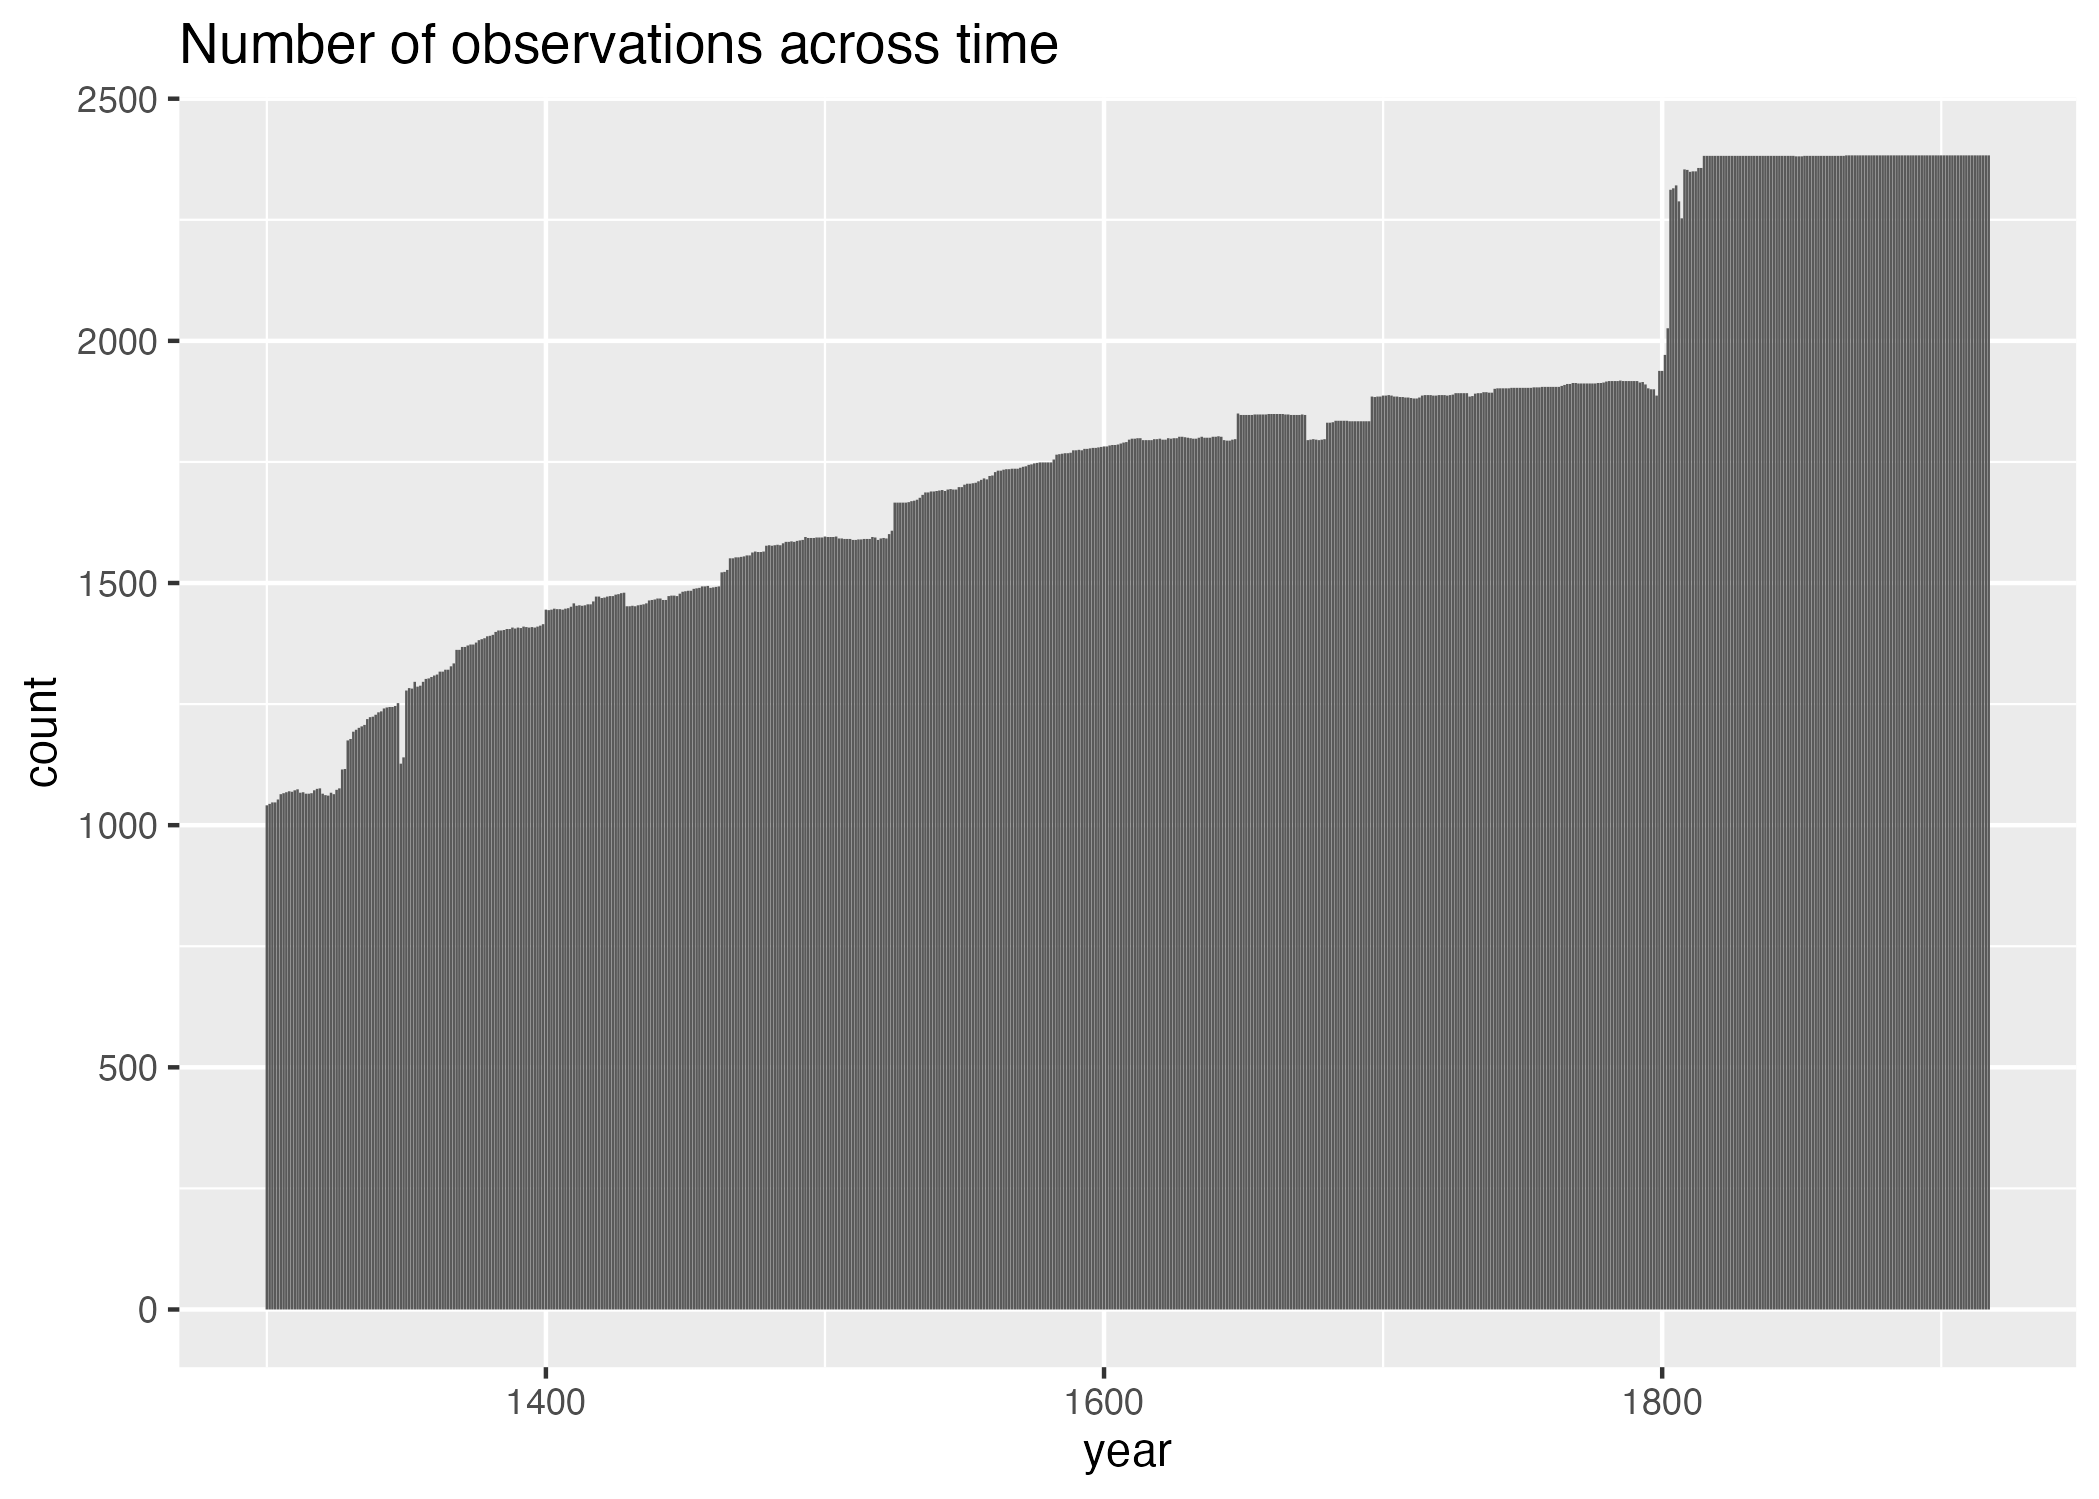
\includegraphics[scale=0.6]{exploration/obs_yearly.png}
    \label{fig:obs_yearly}
\end{figure}
\end{frame}

\begin{frame}
\frametitle{No. of lineages}
\begin{figure}
    \centering
    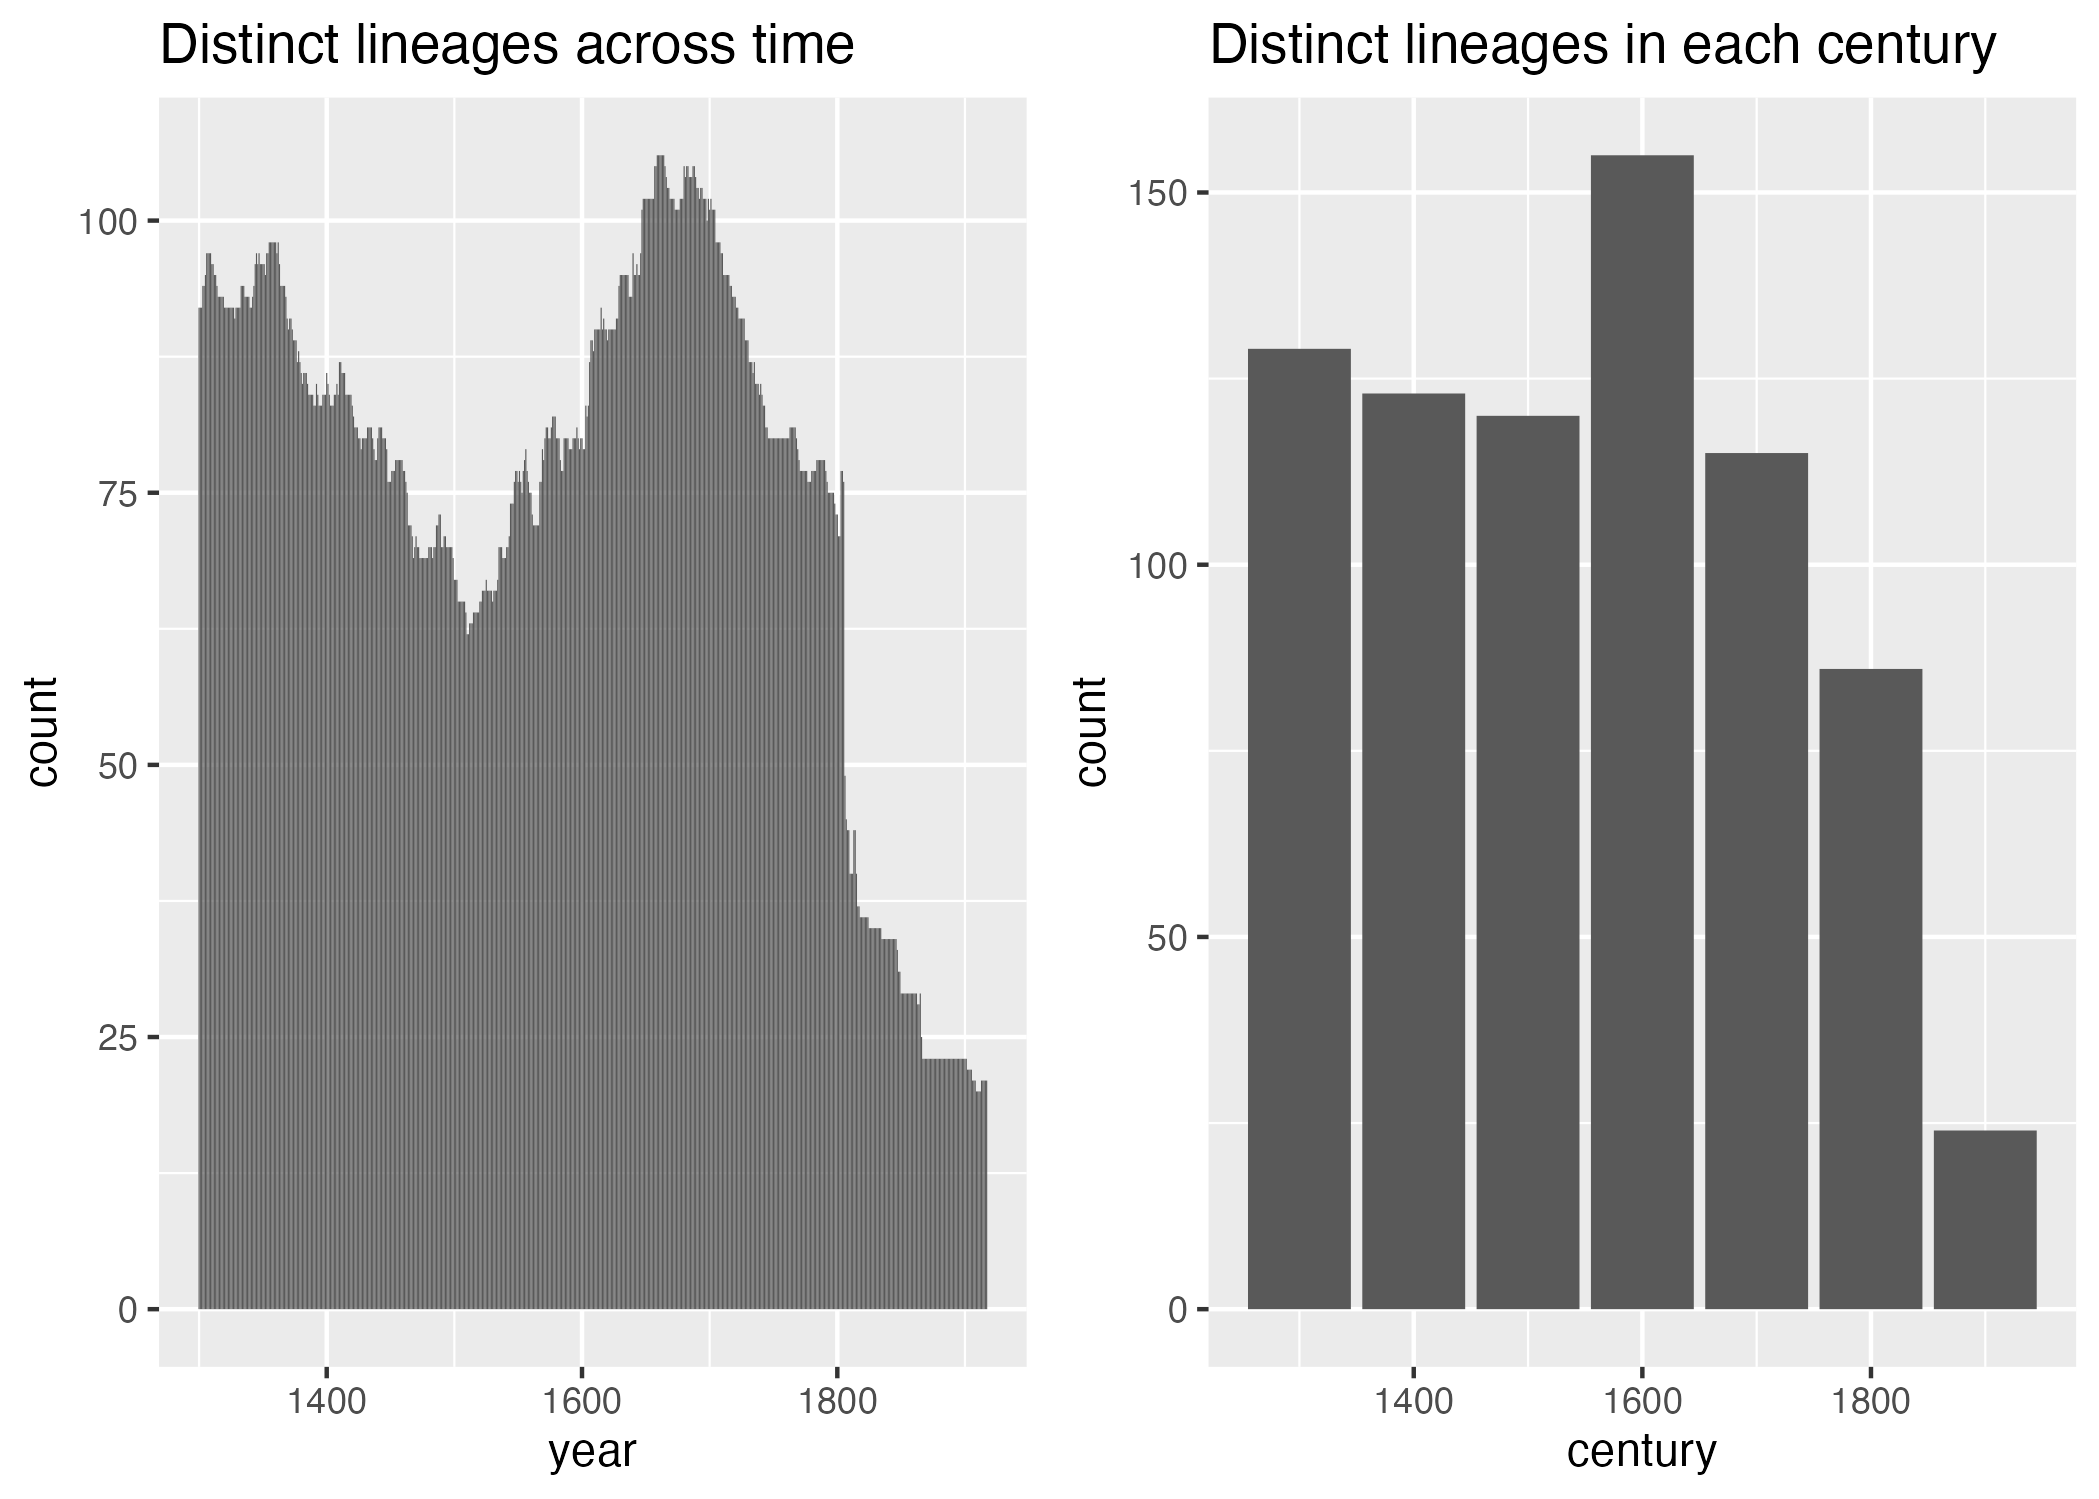
\includegraphics[scale=0.55]{exploration/terrs_yearly_cents.png}
    \label{fig:terrs_yearly_cents}
\end{figure}
\end{frame}

\begin{frame}
\frametitle{Distribution of territory size}
\begin{figure}
    \centering
    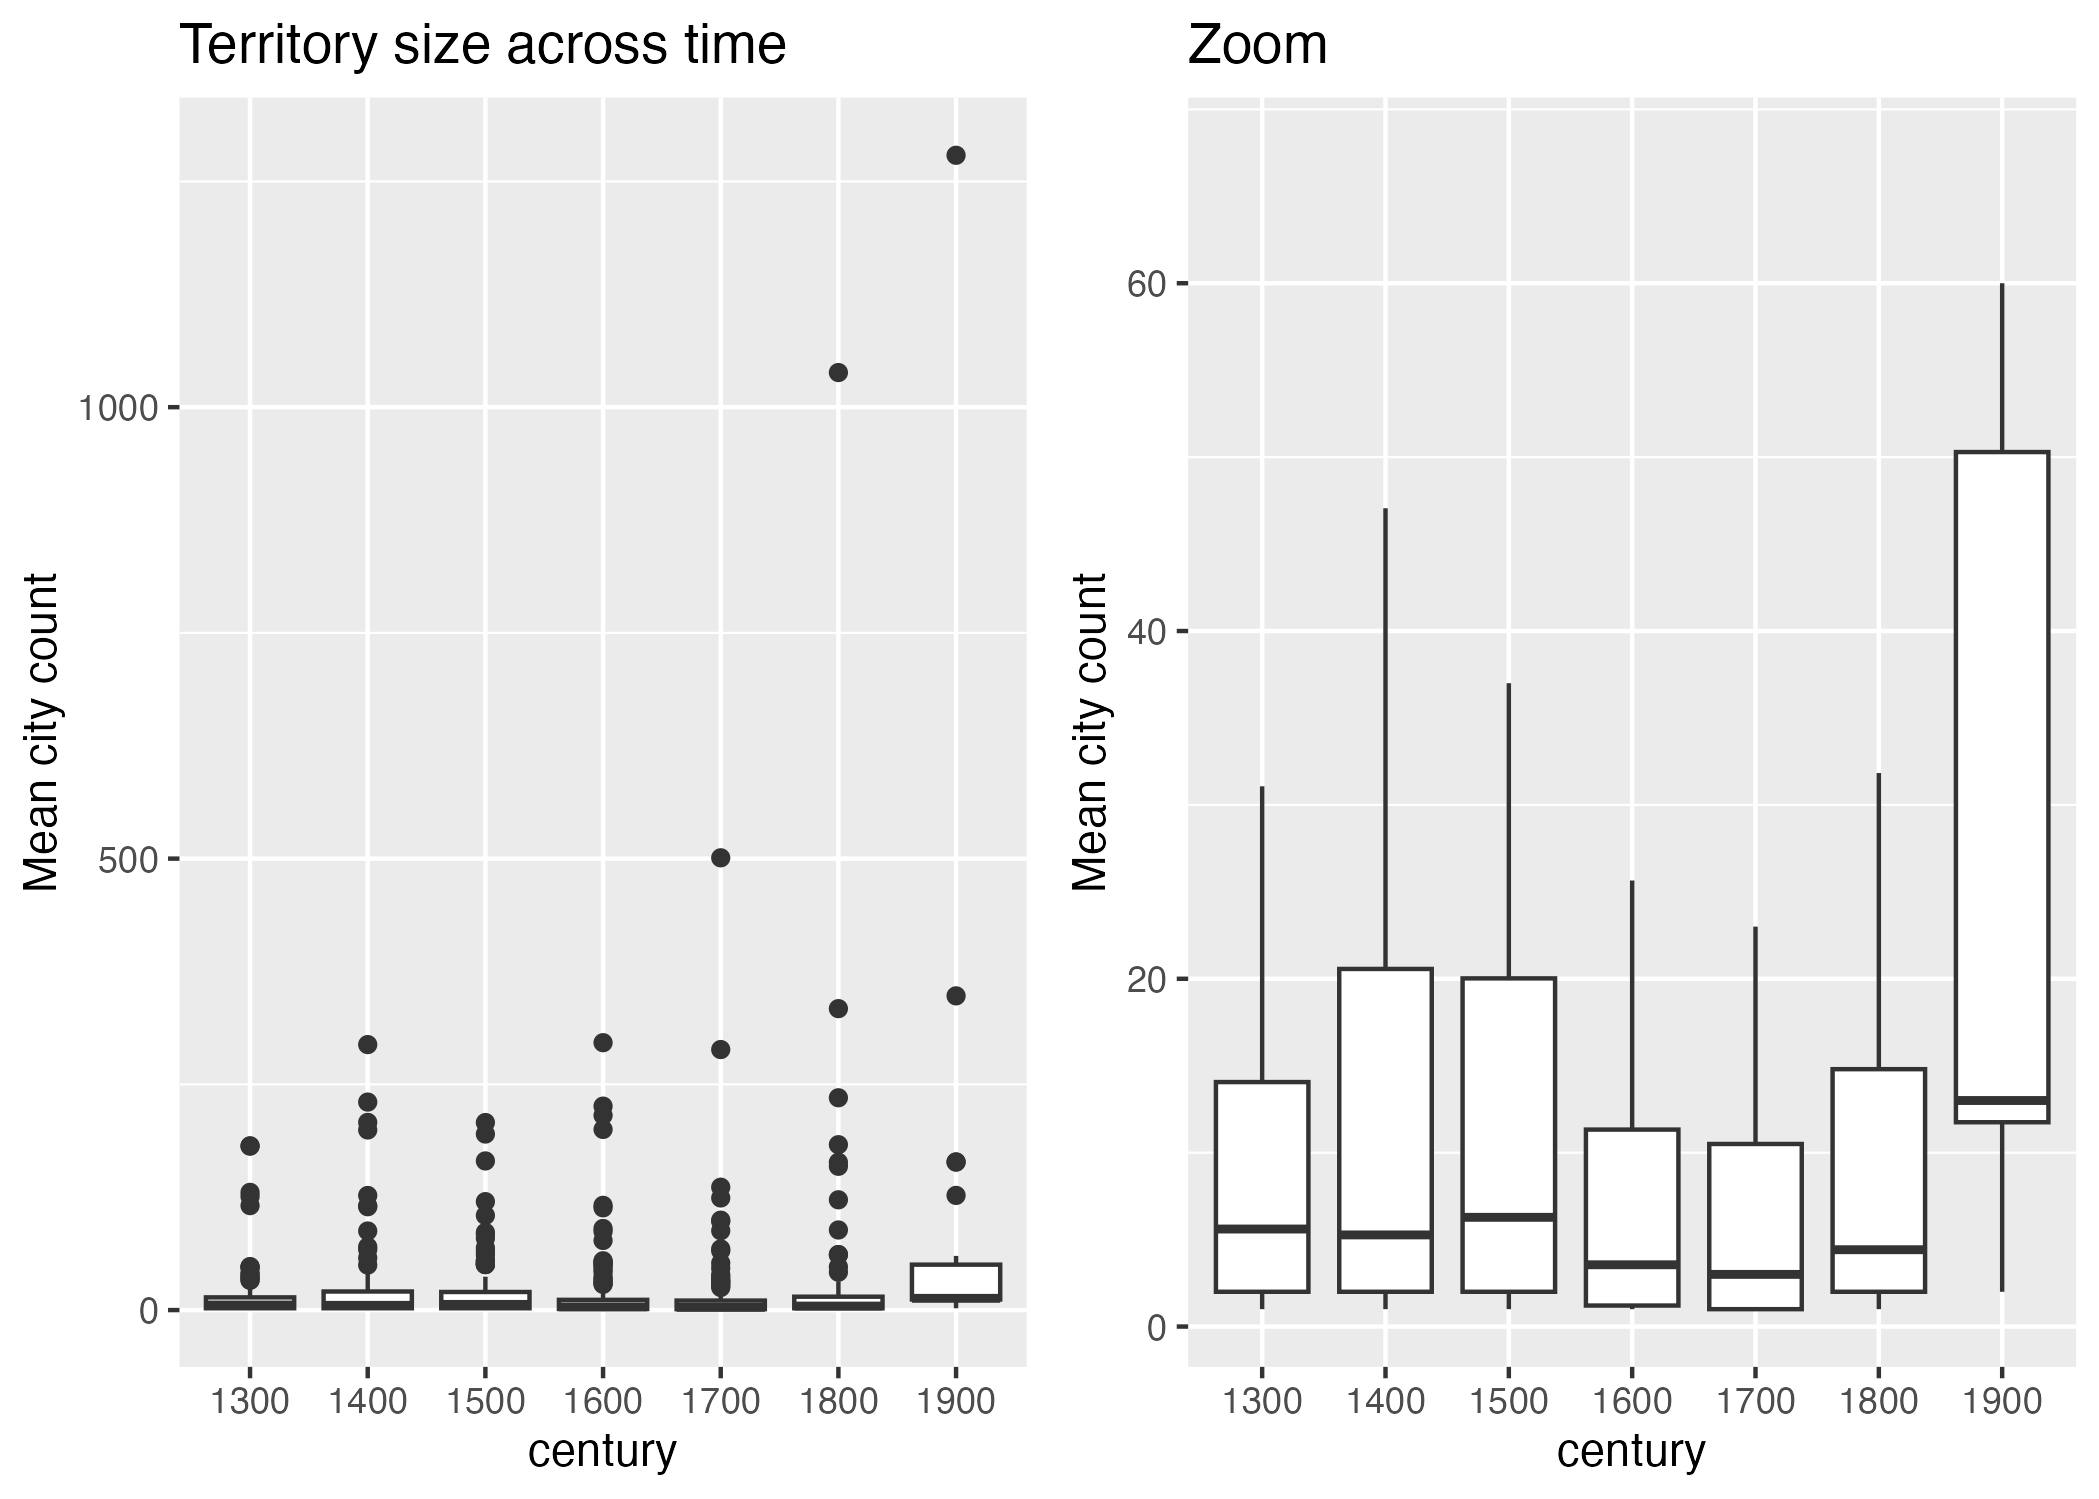
\includegraphics[scale=0.55]{exploration/terrsize_cents_boxplot.png}
    \label{fig:terrsize_boxplot}
\end{figure}
\end{frame}

\begin{frame}
\frametitle{Political integration of cities}
\begin{figure}
    \centering
    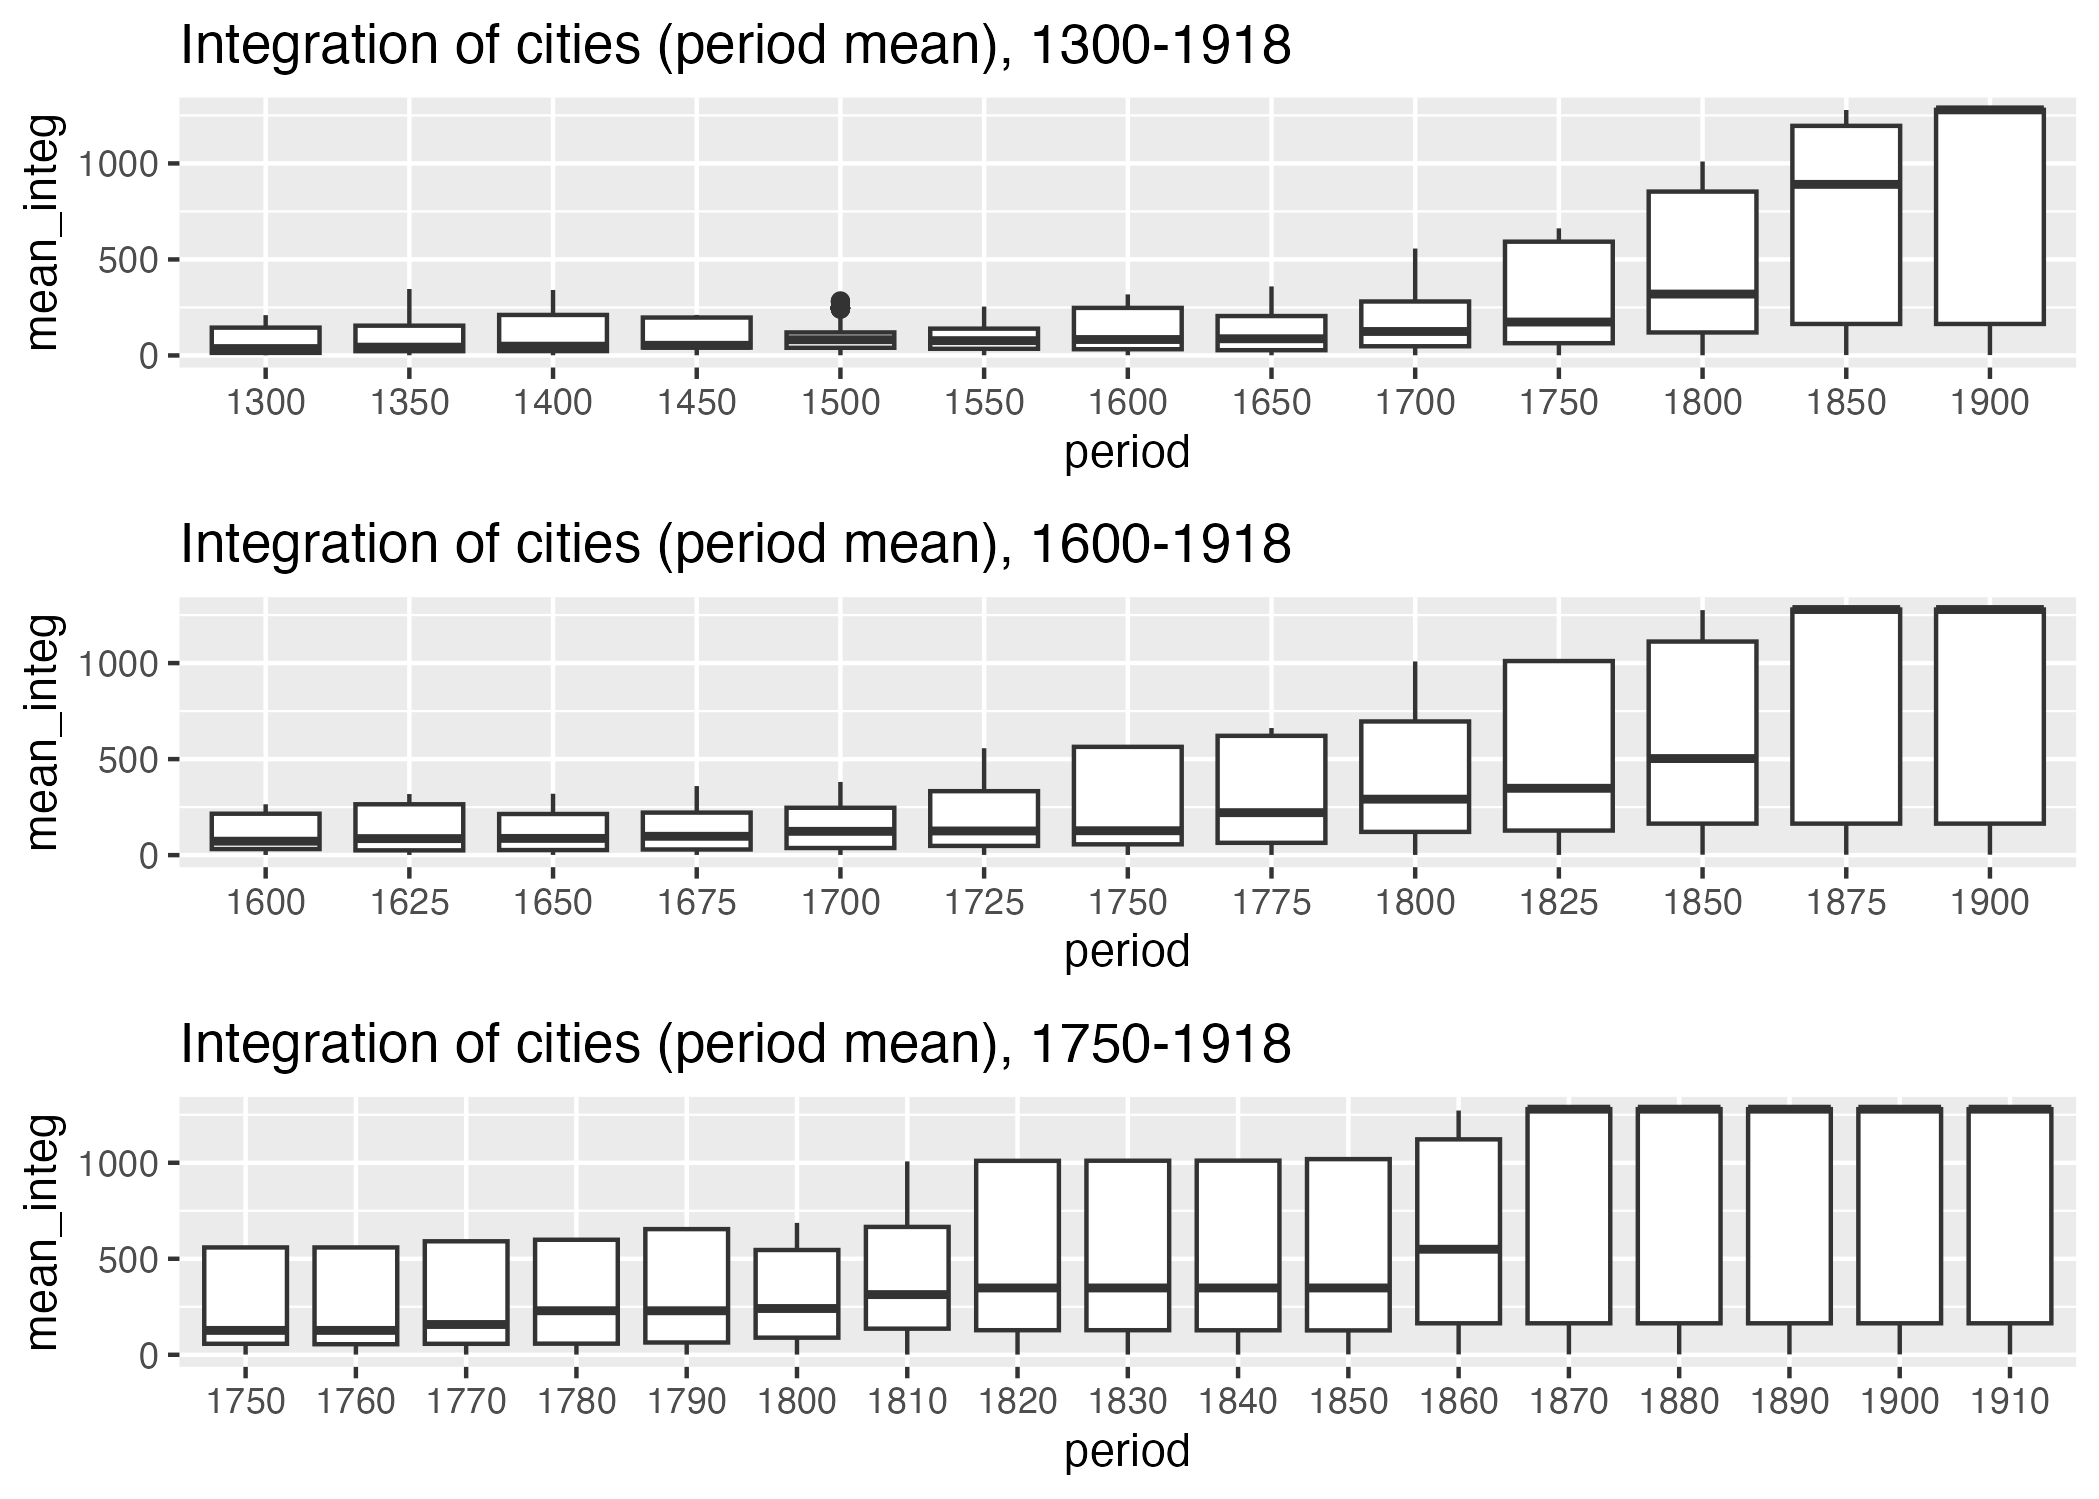
\includegraphics[scale=0.55]{exploration/city_integ_boxplots.png}
    \label{fig:city_integ}
\end{figure}
\end{frame}

\begin{frame}
\frametitle{Lineage extinction events}
\begin{figure}
    \centering
    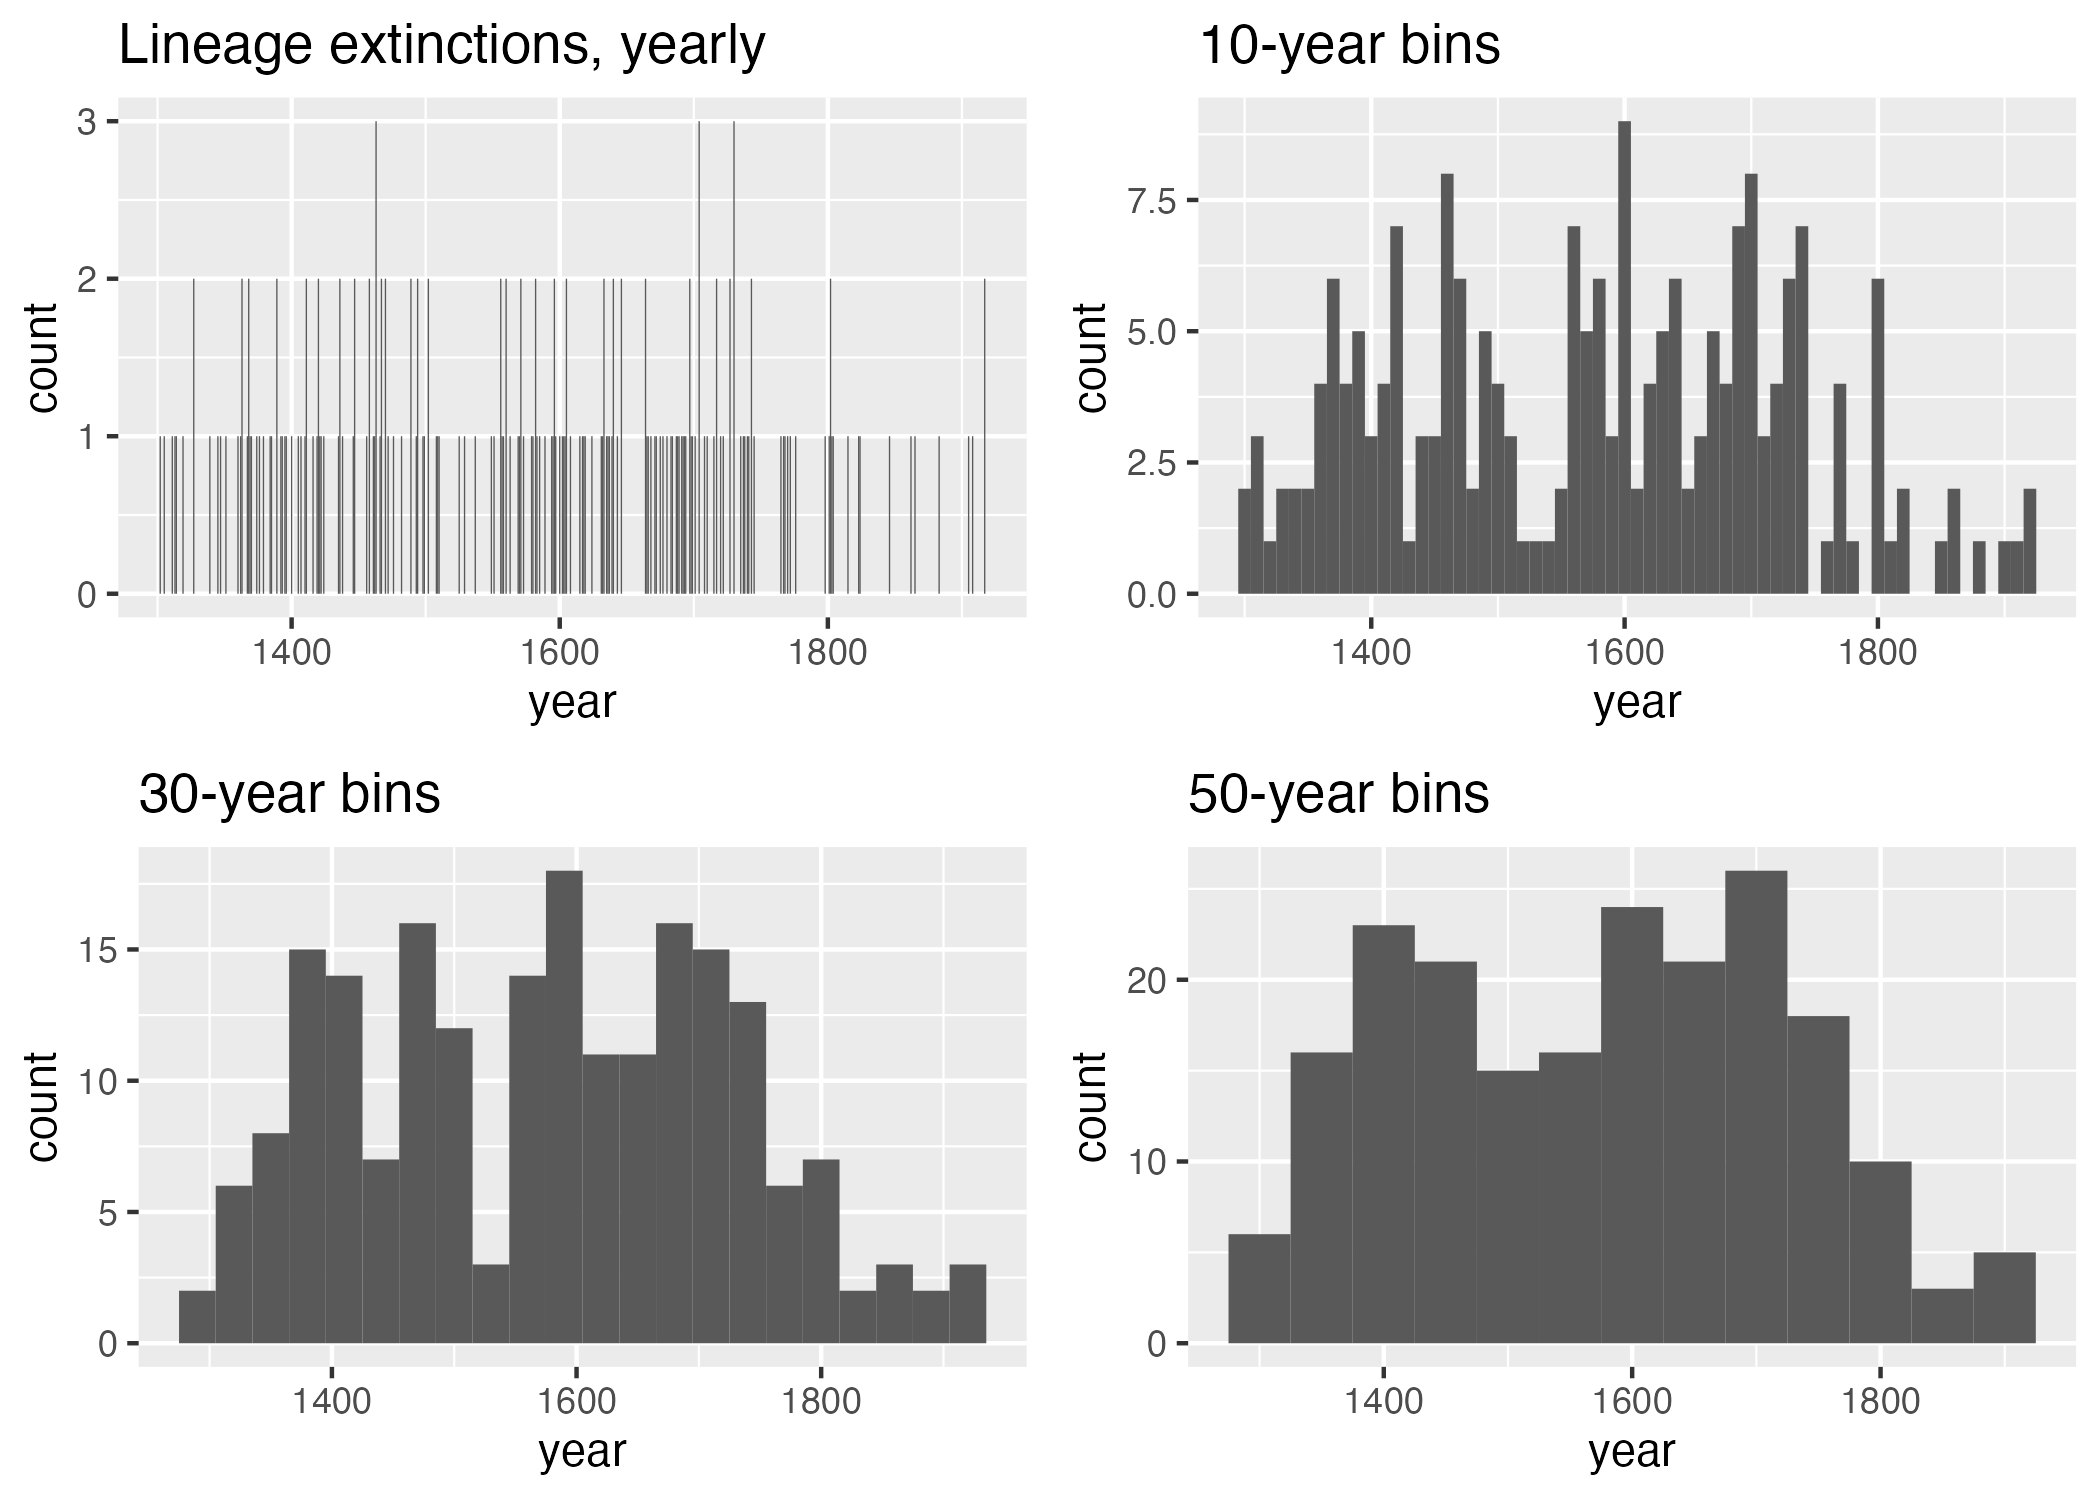
\includegraphics[scale=0.55]{exploration/terrs_ext.png}
    \label{fig:terrs_ext}
\end{figure}
\end{frame}

\begin{frame}
\frametitle{Staggered adoption diff-in-diff}
Estimate the following regression equation:
\begin{equation}\label{eq:did}
\begin{split}
    construction_{itd} = \theta_{id} + \delta_{td} + \beta (Treat_{id} \times Post_{td}) + X_{itd} \Gamma + \epsilon_{itd}
\end{split}
\end{equation}
\end{frame}

\begin{frame}
\frametitle{Sub-experiments}
\begin{figure}
    \centering
    \includegraphics[scale=0.5]{exploration/subexps.png}
    \caption{Assignment of cities to sub-experiments}
    \label{fig:subexps}
\end{figure}
\end{frame}

\begin{frame}
\frametitle{Outcome variables}
\begin{figure}
    \centering
    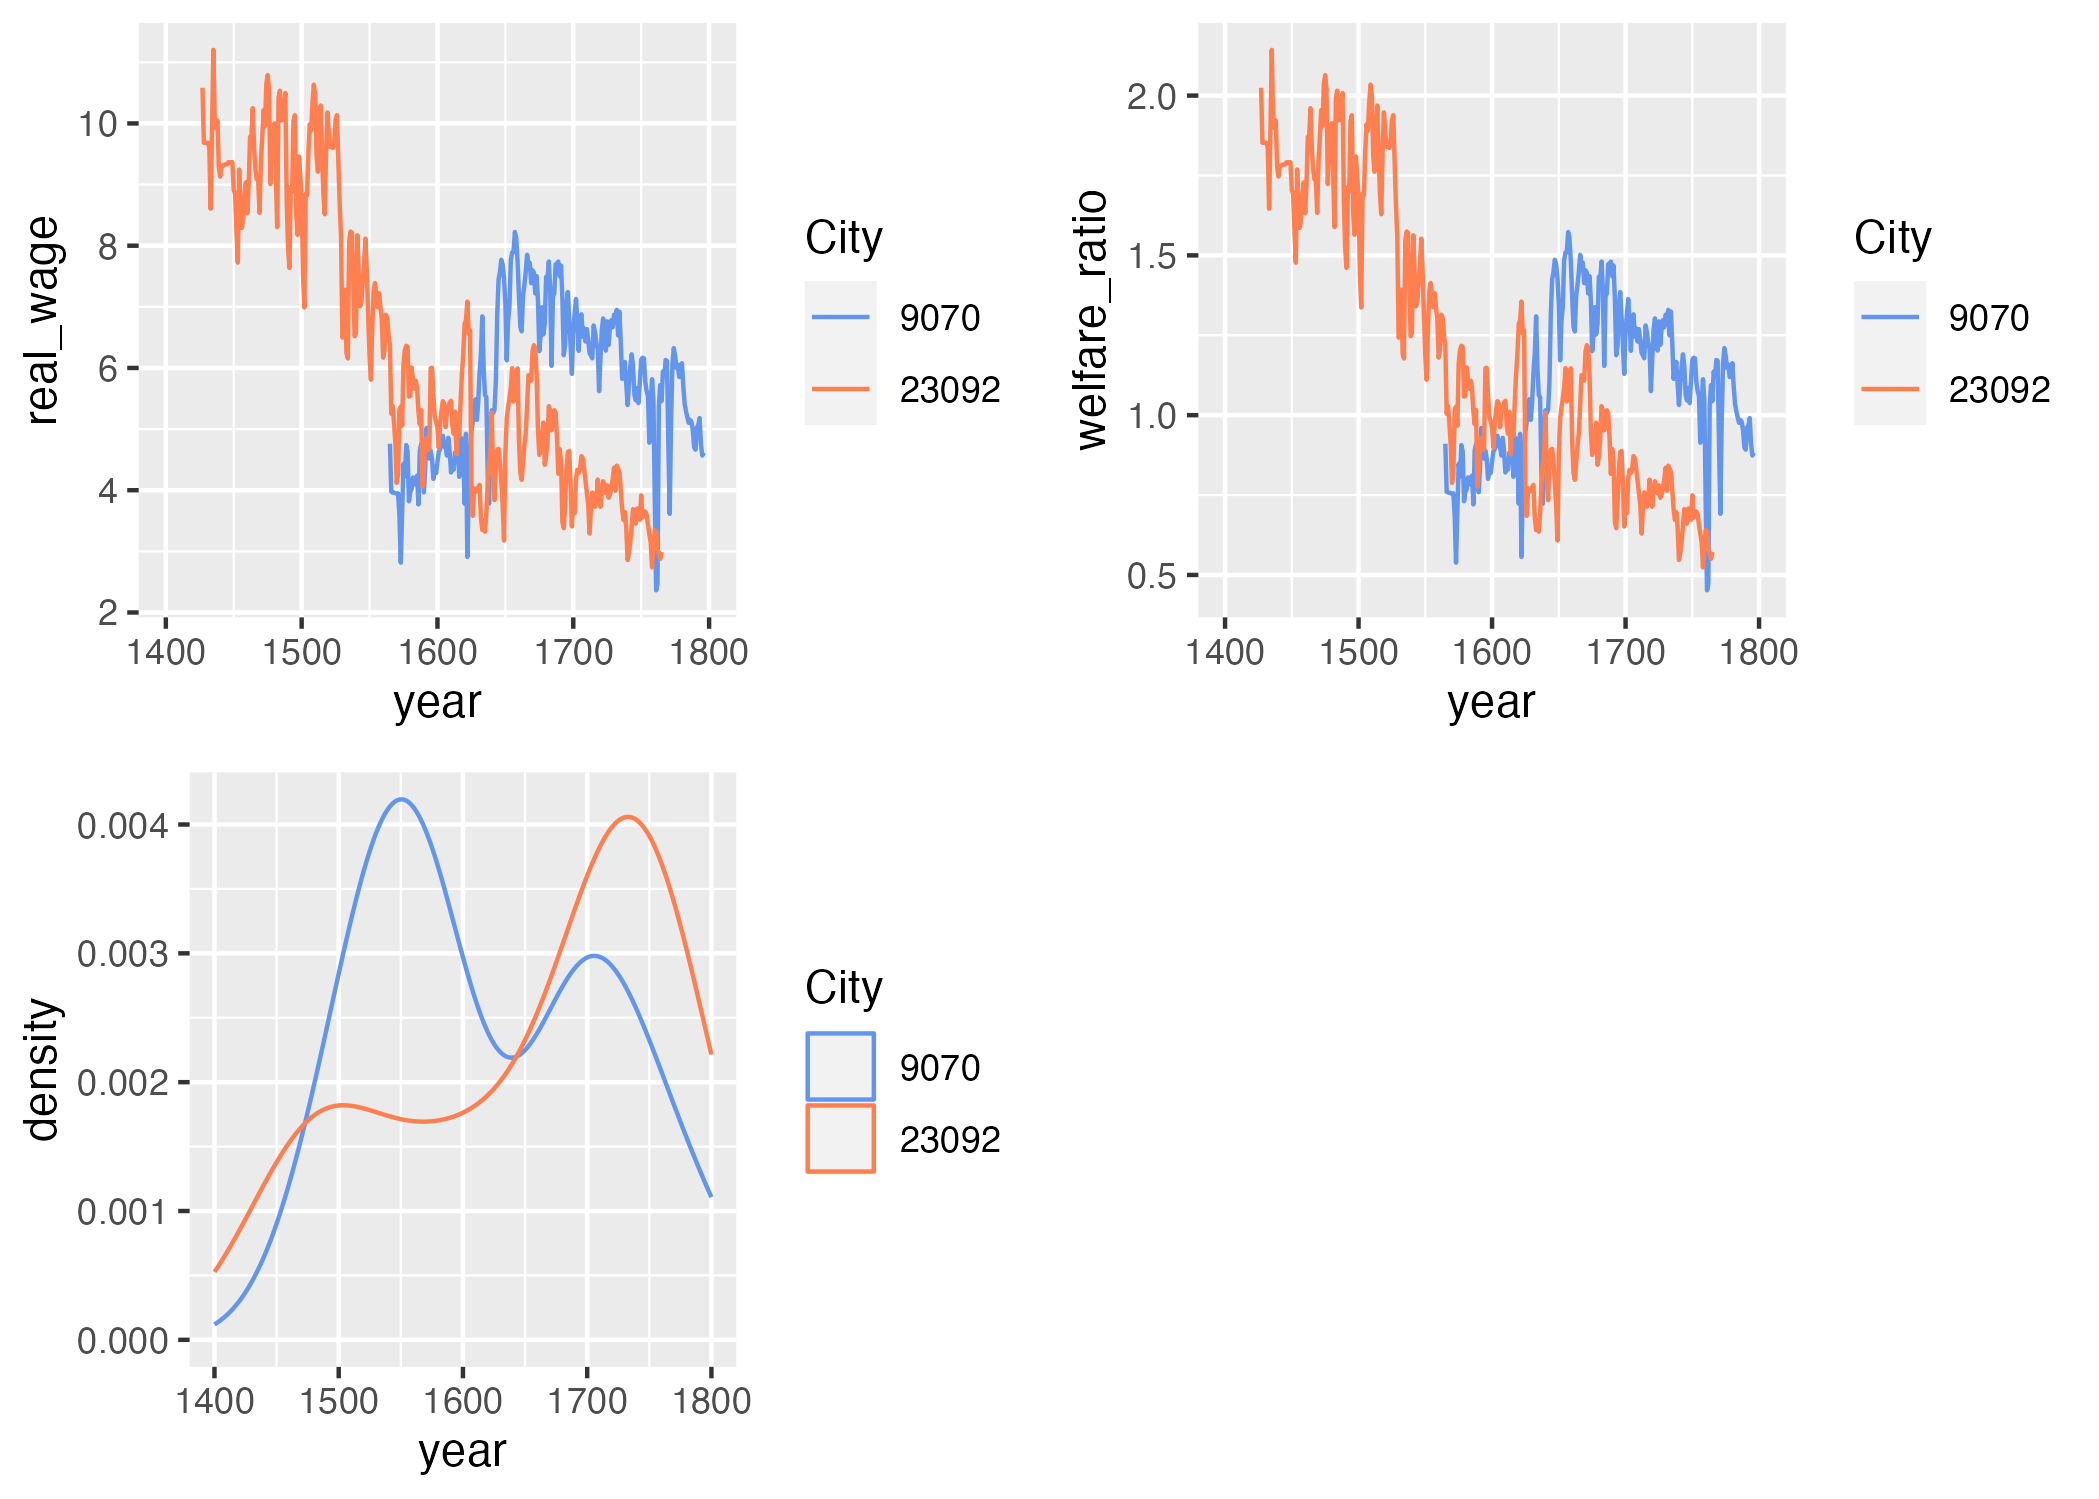
\includegraphics[scale=0.52]{exploration/const_wages.png}
    \caption{Outcomes for Gdansk (1013), Leipzig (9070), and Munich (23092)}
    \label{fig:const_wages}
\end{figure}
\end{frame}

\section{Ideas}

\begin{frame}
\frametitle{Ideas on how to proceed}
\begin{itemize}
    \item double down on the original concept and write that paper, using construction as the outcome
    \item write an econometrics paper on staggered adoption designs, and use what I've got so far as a demonstration / application
    \item use different outcome data?
\end{itemize}
\end{frame}


\begin{frame}
\Huge{\centerline{The End}}
\end{frame}

\section{References}

\begin{frame}
\frametitle{References}
\justifying

\bibliography{references.bib}
\bibliographystyle{chicago}

\end{frame}


\section{Appendix}

\begin{frame}
\frametitle{Appendix: More summary stats}
\begin{figure}
    \centering
    \includegraphics[scale=0.3]{exploration/build_summary.png}
    \label{fig:build_sum}
\end{figure}
\end{frame}

\begin{frame}
\frametitle{Cities affected by extinction events}
\begin{figure}
    \centering
    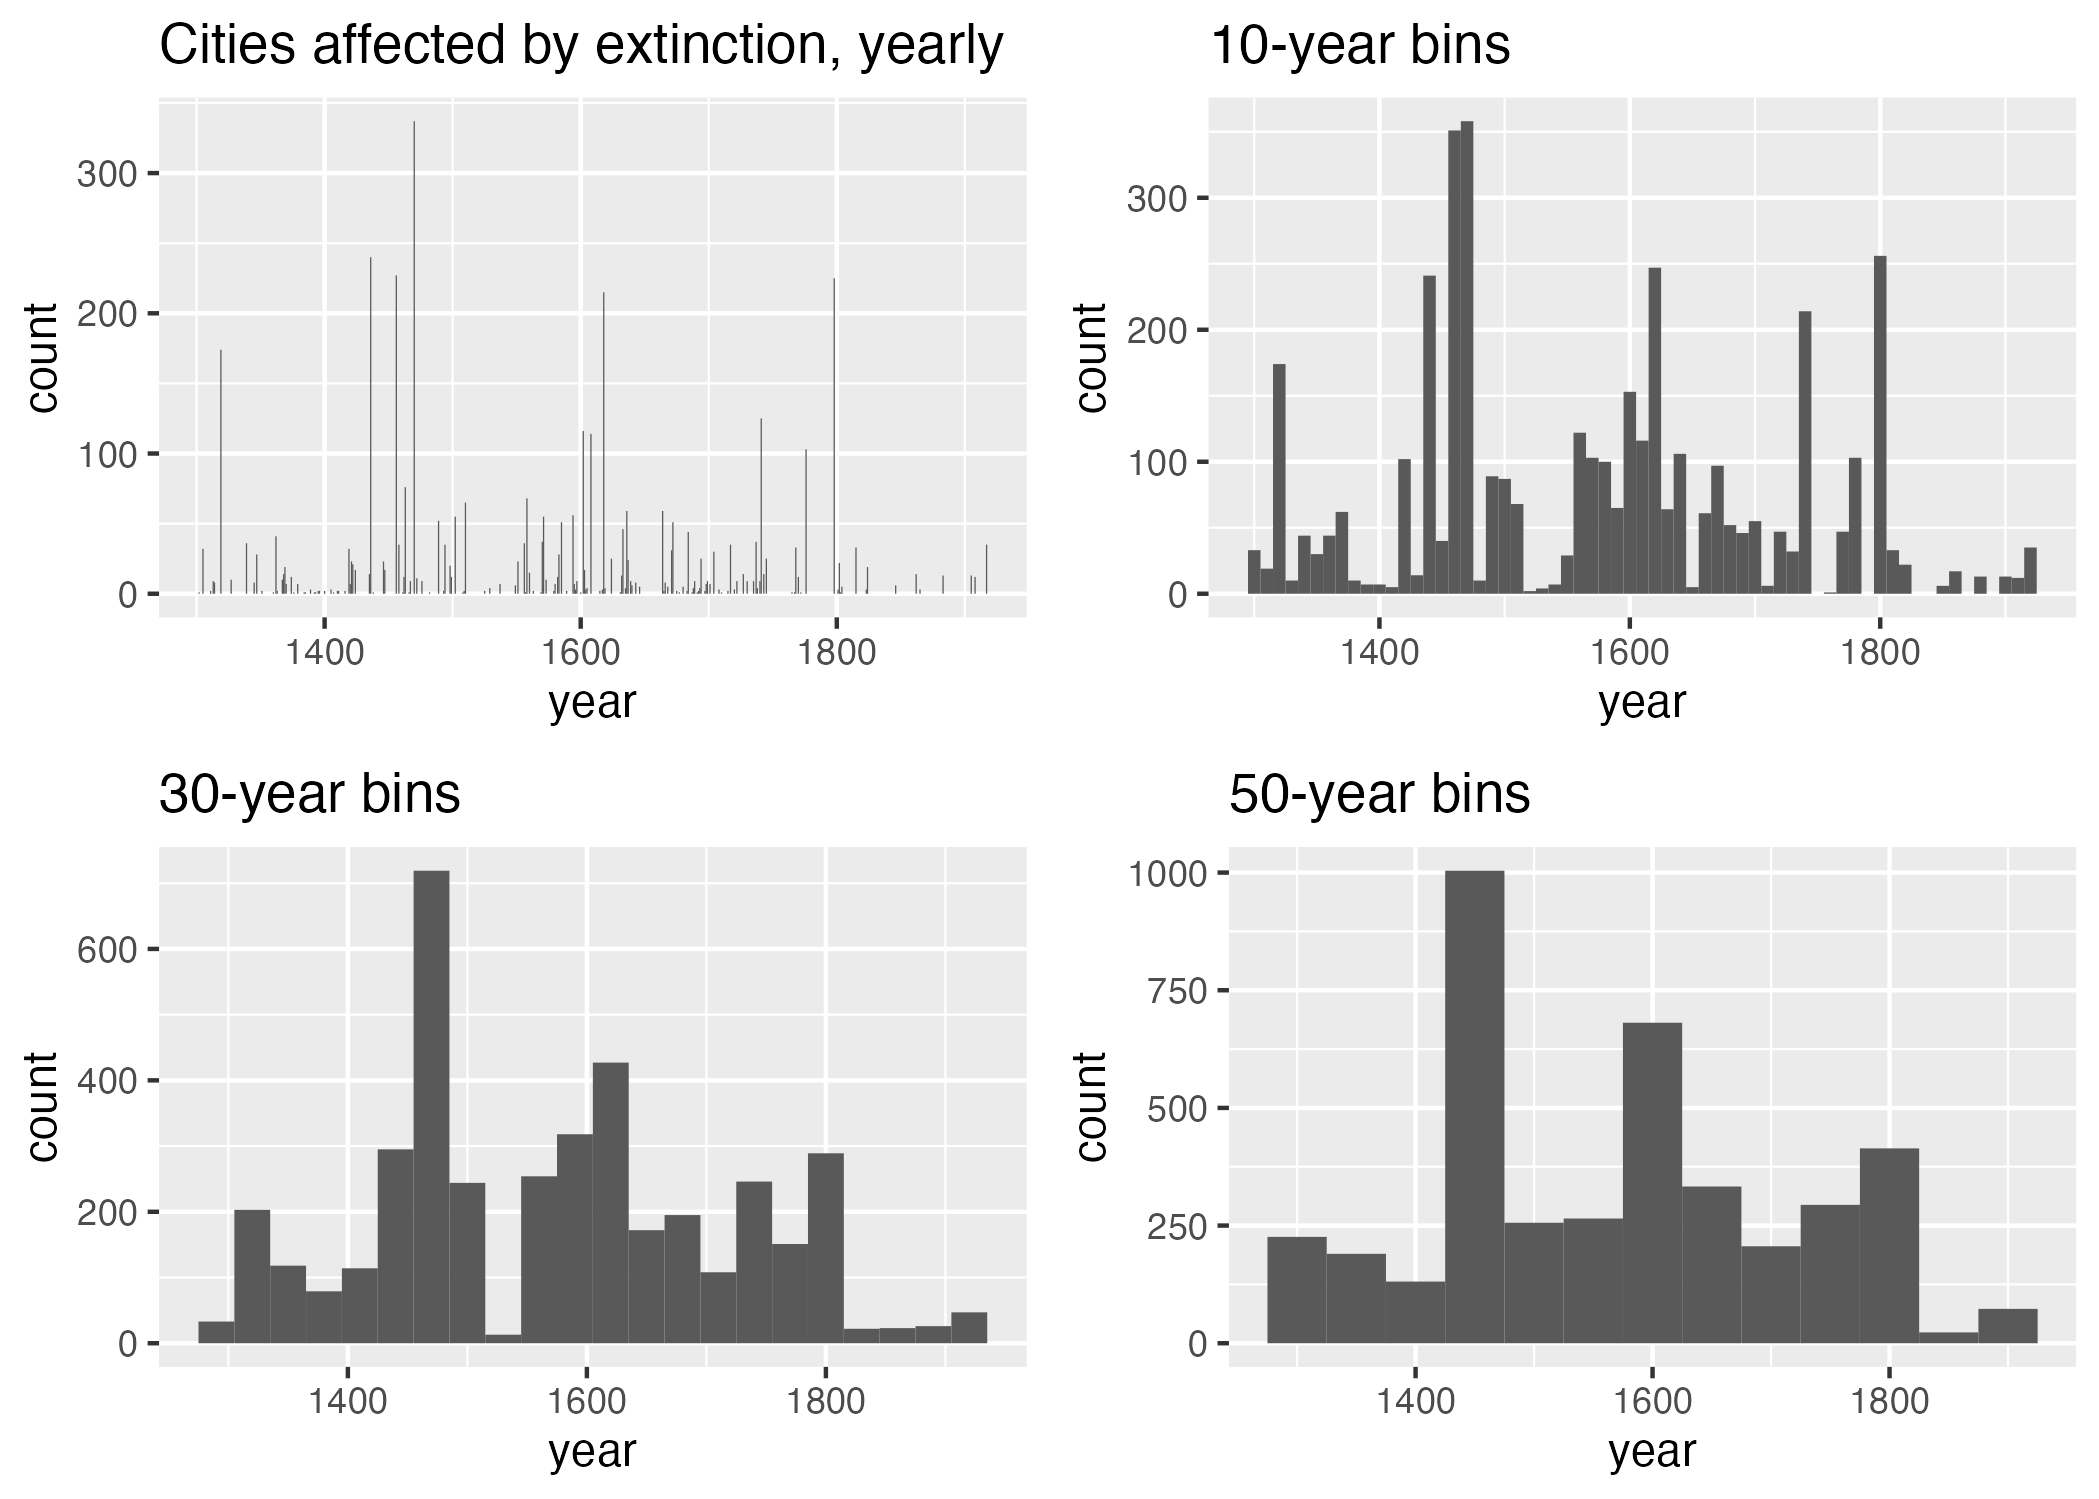
\includegraphics[scale=0.55]{exploration/cities_ext.png}
    \label{fig:cities_ext}
\end{figure}
\end{frame}

\begin{frame}
\frametitle{More summary stats}
\begin{figure}
    \centering
    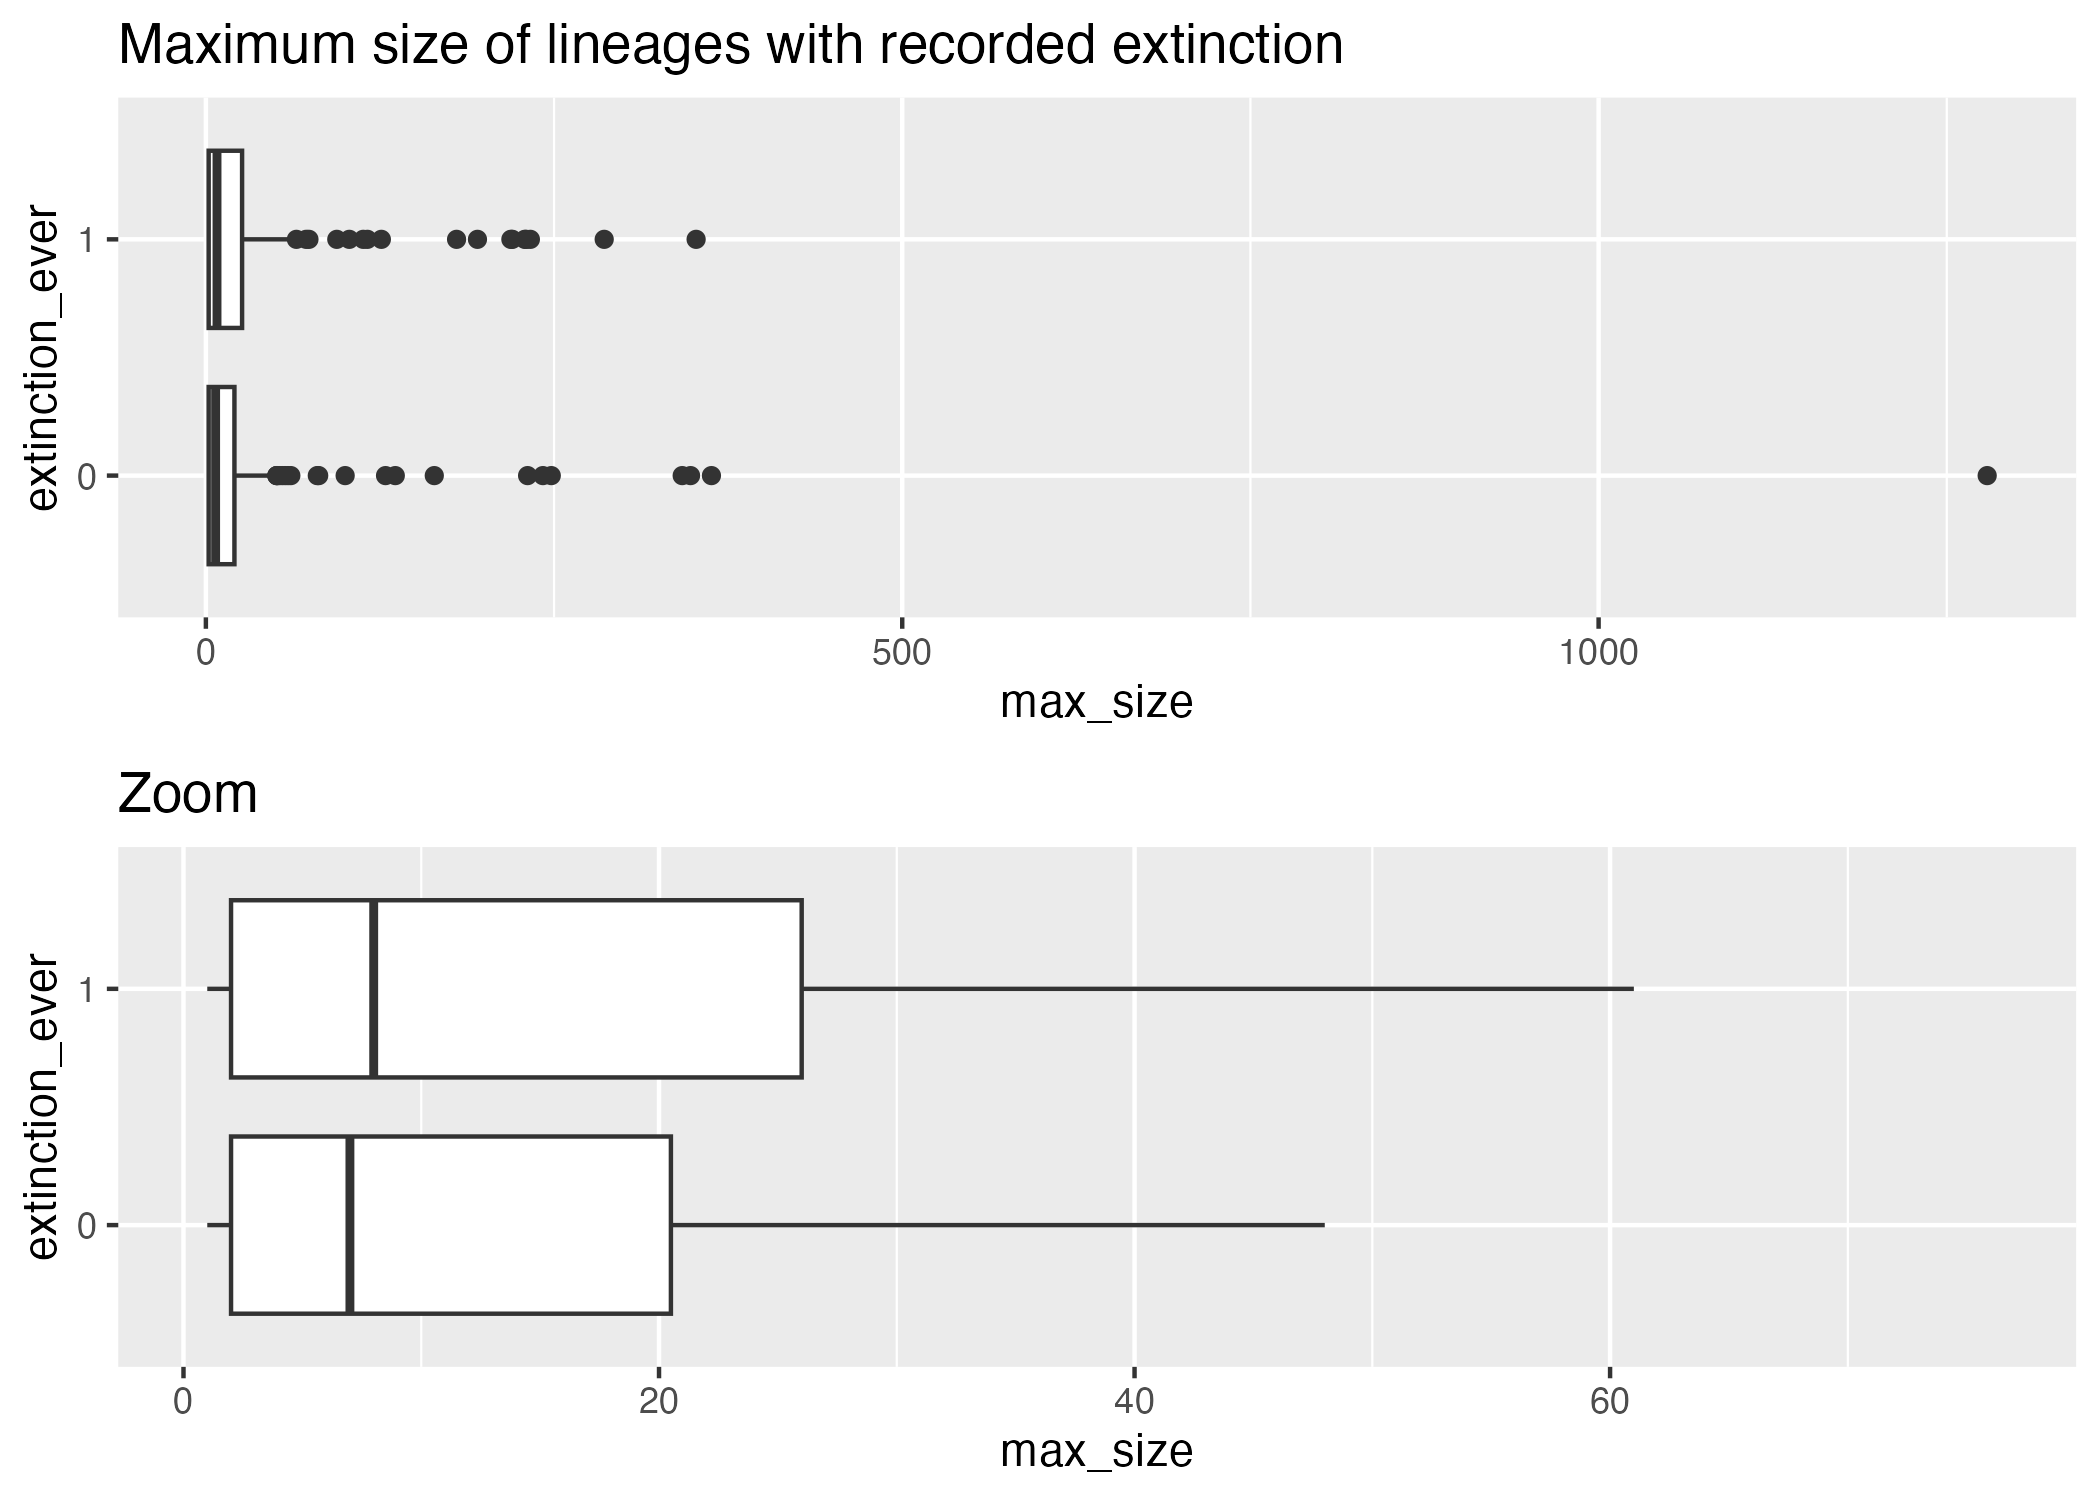
\includegraphics[scale=0.55]{exploration/ext_max_size.png}
    \label{fig:ext_max_size}
\end{figure}
\end{frame}

\begin{frame}
\frametitle{Stacked event study + IV spec}
\begin{equation}\label{eq:eventstudy}
\begin{split}
    construction_{itd} = \theta_{id} +  \sum_{\tau=-10}^{10}\beta_\tau \times I(TSE_{td}=\tau) + \\
    \sum_{\tau=-10}^{10} \delta_\tau \times (\widehat{treat}_{id} \times I(TSE_{td}=\tau)) + X_{it} \Gamma + \epsilon_{it}
\end{split}
\end{equation}
\bigskip
\begin{equation}\label{eq:firststage}
    \widehat{treat}_{id} = \alpha_d + \phi \times I(extinction_{id}) + X_{id} \Gamma + u_{id}
\end{equation}
\end{frame}

\begin{frame}
\frametitle{Example construction series}
\begin{figure}
    \centering
    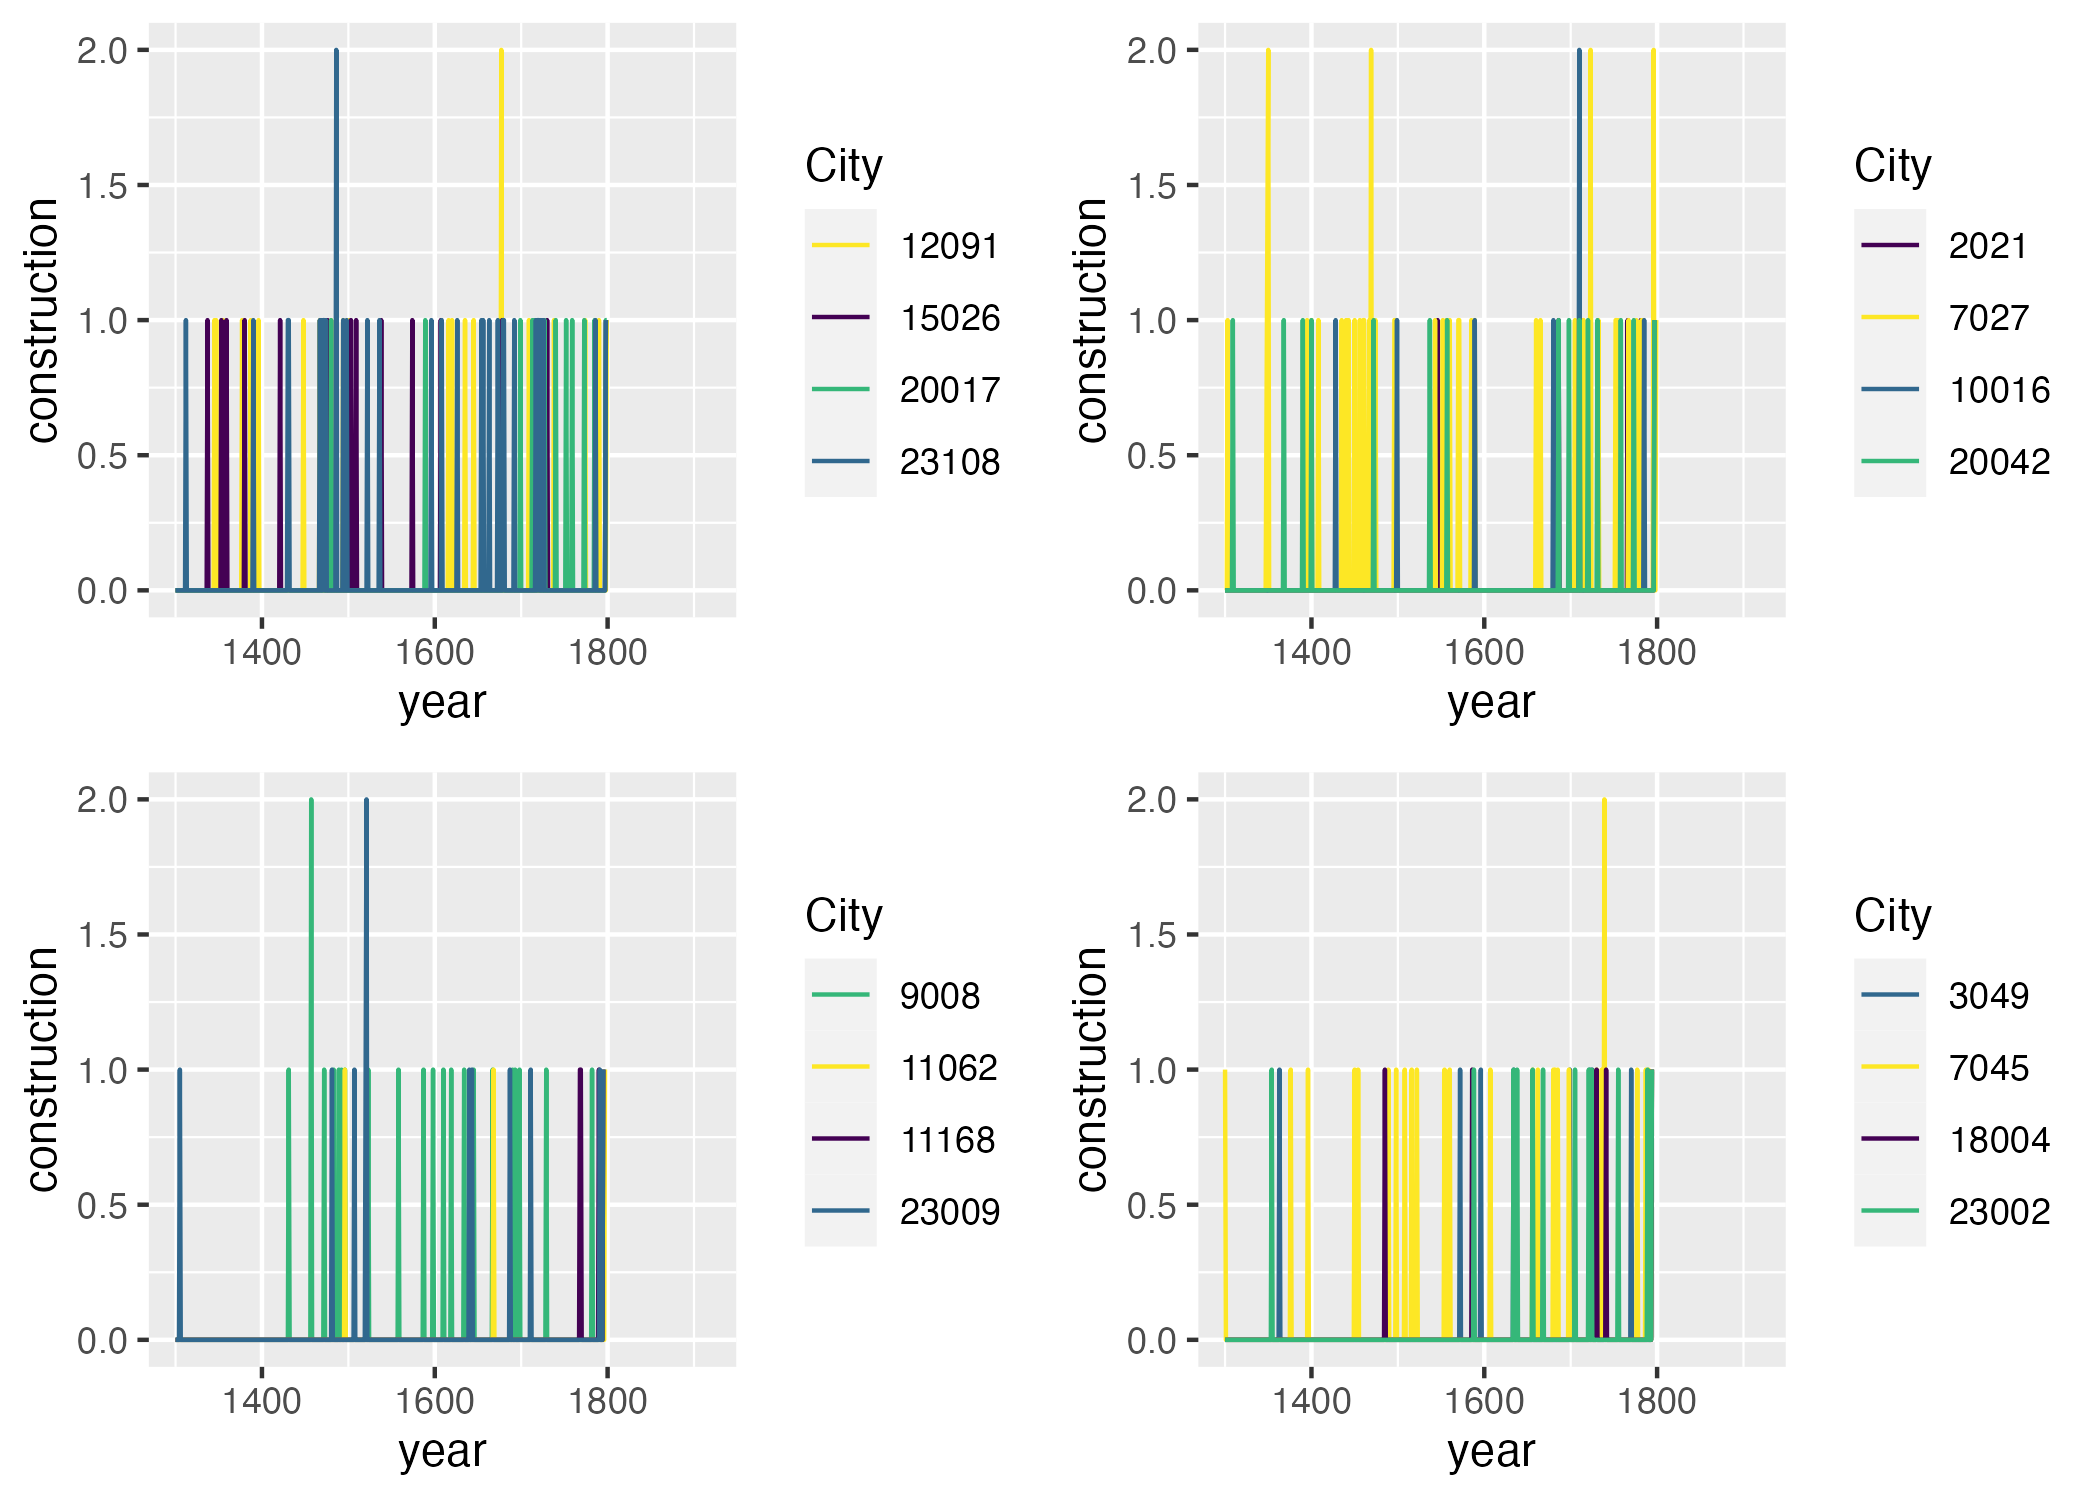
\includegraphics[scale=0.52]{exploration/const_four.png}
    \caption{Construction time series for the 16 cities with the most observations}
    \label{fig:const_four}
\end{figure}    
\end{frame}

\end{document}